\documentclass{article}
\usepackage{extramarks, fancyhdr, minted}
\usepackage{main}

\pagestyle{fancy}
\lhead{\nouppercase{\lastleftmark}}
\rhead{\nouppercase{\lastrightmark}}

\font\manual=manfnt
\def\refname{References}
\def\danger{{\manual\char127}}

\title{SAST\,2023 Summer Training\\CTF | A Warmup for Linux \& Git}
\author{jkjkmxmx @ yhx-12243}
\setdate{2023}{7}{9}

\begin{document}
	\maketitle
	\let\labelitemi\labelitemiii

	\section{Linux}

	\subsection{Introduction}

	\subsubsection[什么是 Linux]{什么是 Linux\protect\cite{net9-linux}}

	Linux 是一种自由和开放源码的类 UNIX 操作系统,其内核由 Linus Torvalds 在 1991 年发布。

	Linux 也是自由软件和开放源代码软件发展中最著名的例子,只要遵循 GNU,任何个人和机构都可以自由地使用 Linux 的所有底层源代码,这使得它得到来自全世界软件爱好者和组织的开发支持。

	Linux 以各种形式被广泛应用在各个领域,包括但不限于:
	\begin{itemize}
		\itemsep0pt
		\item 服务器、主机、超级计算机;
		\item 嵌入式系统(机顶盒、移动设备等);
		\item 基础设施(红绿灯、工业传感器)。
	\end{itemize}

	\subsubsection{发行版}

	我们平时使用的 ``Linux'' 严格来说是 Linux 发行版本,而 Linux 狭义上单指操作系统的内核。

	发行版本在内核的基础上还包括安装工具、系统配置、图形桌面界面、各种 GNU 软件等,使得这个系统能够适用于各种使用目的。

	常见的 Linux 发行版有 Debian、Ubuntu、Fedora、CentOS、Arch Linux 等。不同的发行版使用的软件不同,有些发行版本是设计成专门的目的(比如 Kali 用于网安)。\cite{net9-linux}

	以 Ubuntu 为例,Ubuntu 在每个偶数年的 4 月 (每两年) 发布一个长期支持版 (\textcolor{fuchsia}Long-\textcolor{fuchsia}Term \textcolor{fuchsia}Support),每 6 个月发布一个版本。

	我们提供的服务器安装的发行版是 Ubuntu 22.04 (LTS),代号 Jammy Jellyfish。

	\subsubsection{接触 Linux 的方式}

	我们接触 Linux 的方式通常有以下几种:\cite{net9-linux}

	\begin{itemize}
		\itemsep0pt
		\item 安装 Linux 系统 (单系统、Windows \& Linux 双系统);
		\item WSL (英语:Windows Subsystem for Linux);
		\item 虚拟机 (Virtualbox、Docker);
		\item 服务器远程连接 (SSH、RDP);
	\end{itemize}

	有条件的同学可以给电脑装一个 Linux 系统 (或双系统),\sout{这样你就能在各种配置中度过一段漫长而有趣的时光了}。

	对于其他同学,Windows 的话推荐使用 \href{https://learn.microsoft.com/zh-cn/windows/wsl/install}{WSL\,2} (毕竟是 Type-1 的虚拟机,有性能支持),\sout{如果只想要一个终端的话}\linebreak[1]\sout{可以用 Git Bash};对 macOS 的话原生的终端就有比较接近的体验 (推荐使用 \href{https://iterm2.com/}{iTerm\,2}),或者使用 Docker。当然有服务器的同学可以直接用各种服务器 (现代的服务器基本都是 Linux)。

	\subsection{课前准备}

	参考链接:
	\begin{itemize}
		\itemsep0pt
		\item \url{https://learn.microsoft.com/zh-cn/windows/wsl/install}
		\item \url{https://blog.csdn.net/yushuzhen2008/article/details/104944579}
	\end{itemize}

	\subsection{GUI, CLI, Shell 和 Terminal}

	见 \url{https://docs.net9.org/basic/linux/#basic-concepts}。

	\subsection{学习资料}

	网上的 Linux 学习资料非常多,同学们需要善于寻找资源:

	\begin{itemize}
		\itemsep0pt
		\item \url{https://docs.net9.org/basic/linux/}\quad\textcolor{red}{$\gets$ \textbf{务必熟读,其中的内容本文不再重复出现}}
		\item \url{https://www.runoob.com/linux/linux-tutorial.html}
		\item \url{https://ryanstutorials.net/linuxtutorial/}
		\item \url{https://missing.csail.mit.edu/}
	\end{itemize}

	当遇到问题时,要善于利用 Bing、Google 等搜索引擎,以及 \href{https://stackoverflow.com/}{Stack Overflow}、\href{https://stackexchange.com/}{Stack Exchange} 等。当然在 2023 年的今天,ChatGPT/GPT-4 等工具也一直是你的好伙伴 (对于比较基础的问题效果还是很不错的)。

	当然,在遇到不会的命令时,还要养成看文档的习惯,这一部分可以参考 \hyperref[sss:linuxdoc]{\ref*{sss:linuxdoc} 节}。

	\subsection{Shell}

	Shell 是终端编程中常见的 ``语言'',Shell 变成为典型的命令式编程 (区别于声明性编程),常用于写快餐式的脚本以及充当 ``胶水'' 的作用,\sout{和 Python 比较类似}。

	\subsubsection{Shell 方言}

	Shell 并不是一种固定的语言,它是衍生出的许多方言 (扩展) 的统称,如 \texttt{sh} (原生), \texttt{bash}, \texttt{zsh}, \textcolor{gray}{\texttt{dash}, \sout{\texttt{fish}, \texttt{csh}, \texttt{ksh}}} 等。

	比较常见的是 Bash (Ubuntu 默认) 和 Z shell (zsh, macOS 默认)。当然这些 shell 自身也会有相对应的扩展,比如服务器上默认安装的 Z shell 扩展 \href{https://ohmyz.sh/}{``Oh My Zsh''}。

	通过 \texttt{type} 命令\footnote{有些教程用建议使用 \texttt{which} 命令,但是在有一些 Shell (Sh 和 Bash) 中 \texttt{which} 是\Emm{外部命令},因此无法查阅如 \texttt{if} 等\Emm{内部命令}。而 \texttt{type} 在常见的 Sh, Bash, Z shell 中均为内部命令,可以查询到所有命令的信息。}可见\textcolor{red}{形如 \texttt{cd}, \texttt{if}, \texttt{pwd}, \texttt{alias}, \texttt{setopt}/\texttt{shopt} 等命令返回了 ``shell 内建''/``shell 关键字'',它们统称\Emm{内部命令};而形如 \texttt{ls}, \texttt{wc}, \texttt{ps}, \texttt{cp}, \texttt{find}, \texttt{mkdir}, \texttt{sudo} 等命令会返回一个对应文件所在的路径,它们统称\Emm{外部命令}}\footnote{实际上还有别名,函数等形式,可以使用 \texttt{type -w} (Bash 中为 \texttt{type -t}) 来查看类别。}。% type -w ls cd wc tc if none

	\begin{itemize}
		\itemsep0pt
		\item \Emm{内部命令}是嵌入在各个 Shell 中的 (写在对应的源码里),\sout{就像你们写 Shell 大作业时的一堆 if/else 里讨论的命令},\textcolor{green!80!black}{不创建新进程,执行速度较快},缺点是\textcolor{red}{不同的 Shell 的实现可能会不一样,就是说方言可能会比较多}。
		\item \Emm{外部命令}是 Linux 系统中独立存在的外部程序,\textcolor{green!80!black}{由于是外部程序,因此在所有 Shell 看来表现几乎一样},\textcolor{red}{调用时会创建新的子进程}。

			当输入文件名为一个标识符时,Shell 通常不会解析为相对路径,而是解析为命令,然后按照内部优先,外部其次的顺序进行查找。其中外部命令的查找会根据 \texttt{PATH} 环境变量\textit{按顺序依次查找}。

			具体的优先级可以使用 \texttt{type -a <command>} 来查看,以得知有哪些结果被覆盖。
	\end{itemize}

	\subsection{在 Linux 中查文档}
	\label{sss:linuxdoc}

	在 Linux 以及之后的各种工作中,查文档是必不可少的技能。除上网查询外,Shell 中查文档的方法主要有如下几种:
	\begin{itemize}
		\itemsep0pt
		\item \texttt{<command> --help},\textbf{只能用于 (文档良好的) 外部命令} (大多数外部命令都有良好的文档)。
		\item \texttt{help <command>},\textbf{Bash 中查询内部命令的方式}。
		\color{red}\item \texttt{man <command>},比较通用,\textbf{非常牛逼,非常详细,而且通常由官方撰写的命令手册},强烈推荐使用!

			\normalcolor\texttt{man man} 可以查询 \texttt{man} 的使用方式,\sout{没想到吧,这就叫元学习!}

			所有这些手册 (\texttt{man}ual) 分为 9 类\cite{man-man}:
			\begin{enumerate}
				\item 可执行程序或 shell 命令;
				\item 系统调用 (内核提供的函数);
				\item 库调用 (程序库中的函数);
				\item 特殊文件 (通常位于 \texttt{/dev});
				\item 文件格式和规范,如 \texttt{/etc/passwd};
				\item 游戏;
				\item 杂项 (包括宏包和规范),如 \texttt{man(7)}, \texttt{groff(7)}, \texttt{man-pages(7)} 等;
				\item 系统管理命令 (通常只针对 root 用户);
				\item 内核例程 (非标准)。
			\end{enumerate}

			\compress{-17.5pt}{通过 \texttt{man <\kern0pt类别\kern0pt> <\kern0pt命令\kern0pt>} 可以具体指定在哪一类中查。大家可以体会一下 \texttt{man 1 printf} 和 \texttt{man 3 printf} 的差别\footnote{\url{https://www.cnblogs.com/kelamoyujuzhen/p/9822224.html}, \url{https://blog.csdn.net/weixin_50502862/article/details/125583685}}。}

			另外一个常用的选项是 \texttt{-k},就当你不知道要对什么 \texttt{man} 时,查询所有能匹配正则表达式的手册列表。

			此外,进入手册后,Shell 通常会使用一个叫做 \texttt{less} 的 Pager (说人话就是你和使用 \texttt{less} 命令一样),这是一个和 Vim 类似的环境。此时你可以 \texttt{man less} 或直接按下 ``\texttt h'' 键 (或直接搜索) 寻求帮助,比如常见的 ``\texttt /'' 表示搜索。

			有关 \texttt{man} 的更多用法详见 \texttt{man man}。
		\color{fuchsia}\item\phantomsection\label{item:docbuiltin}\texttt{man bash}/\texttt{man builtins} (Bash) 和 \texttt{man zshbuiltins} (Z shell) 用于查询所有内部命令的文档。

			\normalcolor\sout{相信大家也被 Z shell 里没有 \texttt{help} 命令而且 \texttt{man if} 跳出的东西云里雾里所困扰吧(逃}
		\item \texttt{tldr <command>}。对于一些不常用的命令,你不打算花时间精雕细琢地学习,只想快速知道最常见的用法 (范式,模板)。这时,\texttt{tldr} 是一个非常不错的选择。\texttt{tldr} (Too long; didn't read) 提供了一些命令的非常常见的套路用法,以加快你的工作效率。
	\end{itemize}

	{\color{red}\bfseries 注:在这之后提到如果有没出现的 ``前置技能'',就表示建议使用 \texttt{man} 或 \texttt{tldr} 工具进行相关自学。\par
	再次提醒,学会主动查手册是一项非常非常非常重要的技能,之后的命令介绍会非常简略,希望大家学会自己查 \texttt{tldr} 获取主要用法,查 \texttt{man} 获取手册!!!\par
	再次提醒,学会主动查手册是一项非常非常非常重要的技能,之后的命令介绍会非常简略,希望大家学会自己查 \texttt{tldr} 获取主要用法,查 \texttt{man} 获取手册!!!\par
	再次提醒,学会主动查手册是一项非常非常非常重要的技能,之后的命令介绍会非常简略,希望大家学会自己查 \texttt{tldr} 获取主要用法,查 \texttt{man} 获取手册!!!}

	\subsection{SSH 相关}

	\textcolor{properpurple}{[\textit{主要命令:\texttt{ssh}, \texttt{scp}, \texttt{ssh-keygen}, \texttt{ssh-copy-id}}]}

	命令的用法请使用 \texttt{man} 以及 \url{https://docs.net9.org/basic/linux/#ssh} 进行学习。值得注意的一点是,可以在家目录下配置 \texttt{.ssh/config} 文件来将记住常用的服务器配置 (VSCode 也会使用这个!) 详细的规范见 \verb!man ssh_config!。

	\subsection{Shell 语法}
	\label{sss:shell-syntax}

	\textcolor{properpurple}{[\textit{方便起见,本节内容偏向 Z shell。}]}

	见\autoref{table:grammar},扩展自 \cite{lbwvssl}。官方文档可参考 \url{https://zsh.sourceforge.io/Doc/Release/index.html}。

	\begin{table}[H]
		\centering
		\begin{tabular}{|c|c|c|c|}
			\hline
				命令 & 例子 & 介绍 & 手册 \\
			\hline\hline
				\texttt{\# comment} & \texttt{\# this is a comment} & 注释 & \texttt{man zshmisc} \\
			\hline
				\texttt{<VARIABLE>=<VALUE>} & \vbox to16pt{}\vtop to12pt{}\texttt{ANSWER=42} & \parbox{140pt}{定义一个变量,\textbf{\color{red}注意等号两边不能有空格,且Shell 大小写敏感}} & \texttt{man zshparam} \\
			\hline
				\verb!${VARIABLE}! & \verb!echo ${ANSWER}! & 使用变量,无歧义时可省略大括号 & \texttt{man zshparam} \\
			\hline
				\verb!$NUM! & \vbox to18pt{}\vtop to12pt{}\verb!echo $1! & \parbox{140pt}{使用参数,如 \texttt{./script arg1 arg2 arg3} 中 \texttt{\$2} 即为 \texttt{arg2}} & \texttt{man zshparam} \\
			\hline
				\verb!$@! 或 \verb!$*! & \verb!echo $*! & 所有参数的数组 & \texttt{man zshparam}\footnotemark \\
			\hline
				\texttt{expr} & \texttt{expr 2 + 4} & 计算数学表达式 & \texttt{man expr} \\
			\hline
				\verb!`COMMAND`! 或 \verb!$(COMMAND)! & \verb!echo $(expr 2 + 4)! & 取命令结果 & \texttt{man zshexpn} \\
			\hline\hline
				\verb!{A,B,C}! & \verb!cat file{A,B,C}.txt! & 按照分配律展开 & \texttt{man zshexpn} \\
			\hline
				\verb!{low..high}! & \verb!touch test{1..10}.in! & 范围展开 & \texttt{man zshexpn}  \\
			\hline
				\verb!~! & \verb!cd ~! & 展开你的家目录 & \texttt{man zshexpn} \\
			\hline
				\verb!~USER! & \verb!echo ~root! & 展开某个用户的家目录 & \texttt{man zshexpn} \\
			\hline
				\texttt ?, \texttt *, \texttt{**}, \texttt{[...]} & \vbox to18pt{}\vtop to12pt{}\verb!rm **/A?[1-5].log! & \parbox{144pt}{文件名匹配 (\href{https://en.wikipedia.org/wiki/Glob_(programming)}{Glob}) 语法,\textbf{\color{red}使用引号可以避免自动展开} (\texttt{zshmisc})} & \texttt{man zshexpn} \\
			\hline
		\end{tabular}
		\caption{常用语法}
		\label{table:grammar}
	\end{table}

	\footnotetext{不同 Shell 对这种变量的处理方式大相径庭。Bash 的处理比 Z shell 更加混沌邪恶。在 Z shell 中 \texttt{\$*} = \texttt{\$argv},以及对应的 \texttt{\$ARGC},具体区别可见 \texttt{man zshparam}。}其它复杂的语法 (如 \verb!() (()) [] [[]] {} if for case select! 数组、算术运算 定义函数等) 可见 \texttt{man zshexpn},\texttt{man zshparam},\texttt{man zshmisc} 等。\footnote{注:如果你真的想在 Shell 里使用复杂的语法,建议使用 Python 等方便的语言。}

	所有文档可通过 \verb!ls /usr/share/man/man1/zsh*! 或 \texttt{man zshall} 查询,当然也可查询 \url{https://zsh.sourceforge.io/Doc/Release/index.html} (其实内容是一样的说) 或网上相关教程 (不一定靠谱)。

	\subsubsection{环境变量}

	环境变量是一类特殊的变量,有点像局部变量,它的一大特性是\textbf{可以继承给它的子进程},从而广泛应用于外部命令们的参数配置。

	环境变量的定义有如下几种方式:
	\begin{itemize}
		\itemsep0pt
		\item \texttt{export <VARIABLE>=<VALUE>}:定义环境变量。
		\item \texttt{<VARIABLE>=<VALUE> <command>}:在这一条命令中拥有该环境变量,命令结束后变量消失 (\texttt{man zshmisc})。
		\item 使用其它程序设置。
	\end{itemize}

	环境变量可以用程序或 \texttt{unset <VARIABLE>} 清除。

	\begin{itemize}
		\itemsep0pt
		\item \texttt{declare} / \texttt{typeset} 可用于查看所有定义的变量。
		\item \texttt{env} 可用于查看所有定义的环境变量,以及运行相关程序。
	\end{itemize}

	\subsubsection[调用其它脚本]{调用其它脚本\protect\cite{lbwvssl}}

	在 Shell 中调用其它脚本有两种方式:\texttt{source} (简写 \texttt .) 或子 Shell (\texttt{zsh <script>} 或使用 \href{https://en.wikipedia.org/wiki/Shebang_(Unix)}{Shebang}),\textcolor{gray}{当然还有一种方法是通过 \texttt{exec} 直接替换当前进程,由于这个区别比较大就不讨论了}。

	主要区别是:\texttt{source} 方法在本 shell 执行,子 Shell 方法会新建子终端执行。

	脚本中的局部变量定义仅属于执行它的终端。

	\begin{minted}[frame=single,linenos=true,rulecolor=blue,escapeinside=||]{shell}
echo 'ANSWER=42' > script.sh
zsh script.sh # 变量在子终端定义
echo ${ANSWER} # 对本终端,变量不可见
source script.sh # 变量在本终端定义,也可用 . script.sh
echo ${ANSWER} # 变量可见
	\end{minted}

	\subsection[Shell 选项]{\danger\footnote{\danger\vtop to14pt{} 为致敬 Knuth 著的 \TeX book 的符号,表示可以选读的进阶内容。}\ Shell 选项}

	\textcolor{properpurple}{[\textit{方便起见,本节内容偏向 Z shell。}]}

	Shell 选项,有些地方有称之为 Shell 专有变量。

	对 Z shell 而言,手册可在 \texttt{man zshoptions} 中查看,使用 \texttt{setopt} 和 \texttt{unsetopt} 设置。

	\autoref{table:setopt} 列出了一些常用的 Z shell 选项。

	\begin{table}[htb]
		\centering
		\begin{tabular}{|c|c|c|}
			\hline
				选项 & 启用 (\texttt{setopt}) 效果 & 禁用 (\texttt{unsetopt}) 效果 \\
			\hline\hline
				\vbox to16pt{}\vtop to12pt{}\texttt{autocd} & \parbox{140pt}{对于无法解析的命令,看成前面有 \texttt{cd}。如 \texttt{..} 默认成为 \texttt{cd ..}} & 无前述效果 \\
			\hline
				\texttt{interactivecomments} & 在交互式终端中允许使用 \texttt{\#} 注释 & 交互式终端不能注释,脚本中仍可注释 \\
			\hline
				\texttt{glob} & 启用 Glob (\texttt{man zshexpn}) & 禁用 Glob \\
			\hline
				\vbox to24pt{}\vtop to18pt{}\texttt{nomatch} & 对于无法匹配的 Glob 报错 & \parbox{162pt}{对于无法匹配的 Glob,直接原样返回 (建议开启这个,因为有些命令需要原样的 \texttt* 等字符,避免频繁打引号)} \\
			\hline
				\texttt{globdots} & Glob 中 \texttt* 匹配隐藏文件 & Glob 中 \texttt* 不匹配隐藏文件 \\
			\hline
				\texttt{globstarshort} & 使用 \texttt{**} 代替 \texttt{**/*} 递归列举文件\footnotemark & 单纯的 \texttt{**} 等价于 \texttt* \\
			\hline
				\texttt{nullglob} & 对于无法匹配的 Glob,返回空串而不报错会原样返回 & 遵循 \texttt{nomatch} \\
			\hline
				\texttt{extendedglob} & 允许使用更高级的语法 (具体参见 \texttt{man zshexpn}) & 禁用高级语法 \\
			\hline
		\end{tabular}
		\caption{常用的 Z shell 选项}
		\label{table:setopt}
	\end{table}

	\footnotetext{递归列举的功能在 Bash 中需要通过打开 \texttt{globstar} 选项来实现。}
	\begin{itemize}
		\itemsep0pt
		\item 使用不带参数 \texttt{setopt} / \texttt{unsetopt} / \texttt{set -o} / \texttt{set +o} 可以查看所有 Shell 选项。
		\item 使用 \texttt{[[ -o <option> ]]} 可以检查某个 Shell 选项是否设置 (\texttt{man zshmisc})。
	\end{itemize}

	\subsection{一些命令}

	这里还有一些\sout{可能在 Puzzle 中用得到的}命令,具体方法请自行使用 \texttt{man} 和 \texttt{tldr} (记住,他们真的是很好的老师,我已经没什么好写的了)。

	\subsubsection{进程}

	\begin{itemize}
		\itemsep0pt
		\item \texttt{ps} / \texttt{top} / \texttt{htop}:查询进程信息
		\item \texttt{uptime}:查询系统启动时间,用户数以及平均负载 \sout{(其实就是 \texttt{top} 的第一行)}
		\item \texttt{exec}:用接下来的程序替换当前进程
		\item \texttt{kill} / \texttt{killall}:杀死进程
		\item \texttt{... \&} / \texttt{fg} / \texttt{bg} / \texttt{jobs} / \texttt{nohup}:前后台切换,\sout{避免《人类的群星闪耀时》}(查不到怎么用?看看\hyperref[item:docbuiltin]{这里}!)
	\end{itemize}

	\subsubsection{文件系统}

	\begin{itemize}
		\itemsep0pt
		\item \texttt{cat}:输出并连接文件
		\item \texttt{tee}:将输入复制一份 (标准输出和文件)
		\item \sout{\texttt{tac} / \texttt{rev}:花里胡哨地输出文件}
		\item \texttt{stat}:显示文件信息
		\item \texttt{wc}:统计行数等信息
		\item \texttt{sort}:排序
		\item \sout{\texttt{tsort}:拓扑排序}
		\item \texttt{uniq}:去重
		\item \texttt{grep}:搜索文件内容
		\item \texttt{awk} / \texttt{cut} / \texttt{sed}:简单文件处理
		\item \texttt{head} / \texttt{tail}:截取文件 (\texttt{tail -f} 比较有用,通常用于输出日志)
		\item \texttt{du}:显示已用空间
		\item \texttt{df}:显示可用空间
		\item \texttt{less}:友好地展示文件内容 (允许手动滚屏)
		\item \texttt{realpath}:显示经过解析的绝对路径 (所有符号链接均经过解析,从根目录开始)
		\item \texttt{basename} / \texttt{dirname}:分离目录名和文件名
		\item \danger\ \texttt{split}:分裂文件 (用于制作分卷压缩包)
		\item \danger\ \texttt{dd}:拷贝文件的底层接口
	\end{itemize}

	\subsubsection[网络]{网络\protect\cite{lbwvssl}}

	\begin{itemize}
		\itemsep0pt
		\item \texttt{ifconfig} / \texttt{ip}:查询网络配置
		\item \texttt{netstat}:查询连接情况
		\item \texttt{ping}:检查网络是否连通
		\item \texttt{curl} / \texttt{wget}:命令行网络 (HTTP 等协议) 连接
		\item \danger\ \texttt{tcpdump}:抓网络包
		\item \danger\ \texttt{nc}:手动发/听网络包
		\item \danger\ \texttt{dig} / \texttt{nslookup}:DNS 解析
	\end{itemize}

	\subsubsection{其它}

	\begin{itemize}
		\itemsep0pt
		\item \texttt{clear} 清屏
		\item \texttt{history} 查询历史记录
		\item \texttt{ulimit} 修改 Shell 的资源限制
		\item \texttt{alias} / \texttt{unalias} 定义与取消定义别名
		\item \texttt{tar} / \texttt{gzip} / \texttt{gunzip} / \texttt{zip} / \texttt{unzip}:各种不同格式的压缩工具
		\item \texttt{shutdown} / \texttt{halt} / \texttt{reboot}:关机及重启
		\item \texttt{date}:显示或更改系统时间
		\item \texttt{uname}:查询系统相关信息 (\texttt{-a})
		\item \texttt{lsb\_release}:(Ubuntu) 查询版本信息 (\texttt{-a})
		\item \texttt{service} / \texttt{systemctl} 操作系统服务
		\item \texttt w / \texttt{who}:查询登录用户
		\item \sout{\texttt{write}:聊天 (记住 Linux 是多用户操作系统) (可以在上某些课时恶搞让别人终端突然收到消息)}
		\item \sout{\texttt{wall}:广播消息}
		\item \sout{\texttt{factor}:分解质因数}
		\item \sout{\texttt{tty}:查询当前 tty}
	\end{itemize}

	\section{Git}

	\subsection{Introduction}

	在代码开发过程中,总会遇到一些问题。
	代码不知道改了哪里不能运行了,想要回退怎么办?
	多个人同时想对代码进行修改(并行开发),开发完后怎么合并?
	显然,有一个能帮助我们解决这些问题的工具将极大的加快我们开发的速度。
	而这种工具,便是版本控制软件。

	版本控制软件帮助使用者找出:

	\begin{itemize}
		\itemsep0pt
		\item 不同版本之间的差异;
		\item 谁做出了这个修改;
		\item 什么时候做出了这个修改;
		\item 做出修改的人给出的修改理由。
	\end{itemize}

	那么,什么是分布式的版本控制软件呢?
	为了了解清楚,我们需要区分中央版本控制系统 (CVCS) 和分布式版本控制系统 (DVCS) 的区别。

	中央版本控制系统必须同时存在服务端和客户端。
	当进行代码备份时,客户端会向服务端发出请求,并将此次修改的内容发送到服务器当中去,服务端收到请求后,会将代码存储在服务器当中;
	同样当客户端想查看某一个版本的修改内容或者想恢复到某一个版本之时,客户端也会发送请求到服务端,服务在端接收到请求之后会做出相应的处理并返回给客户端。
	也就是说,在业务流程过程中,服务端必须存在,所有请求必须经过服务端的处理。

	分布式版本控制器,主要是将备份的代码以及记录完全独立在本地存储。
	比如说当你想将代码恢复到某一个版本的时候,本地版本控制器不需要依赖网络便可以完成此操作,因为本地版本控制器拥有完整独立的一套控制系统。\cite{net9-git}

	\noindent\hrulefill

	Git 作为世界上最流行的 DVCS,占了开源市场版本控制系统约 $74 \%$ 的份额\footnote{\url{https://openhub.net/repositories/compare}, 2023.7.},其余比较常见的有 svn (CVCS, $22 \%$, 代表者 texlive 等),Mercurial (DVCS, $1 \%$, 代表者 nginx 等)。
	而且,很多 DVCS 或多或少受到 Git 的影响 (如 Mercurial/hg 等),因此学习 Git 也会对之后学其他 DVCS 带来便利,这也是我们学 Git 的理由之一。

	\subsubsection[什么是 Git]{什么是 Git\protect\cite{net9-git}}

	Git 是 Linux 之父 Linus Torvalds 为开发 Linux 内核而建立的一个分布式版本控制软件。

	Git 除了版本控制软件本身的优势以外,还可以:

	\begin{itemize}
		\itemsep0pt
		\item 通过查看 Git history,开发者可以看到一个项目开发的时间线;
		\item 通过 Git branch (分支),开发者可以在不用担心影响主代码的情况下进行开发;
		\item ……
	\end{itemize}

	\pagebreak

	\subsection{课前准备}

	Git 下载 (官网):\url{https://git-scm.com/downloads}

	Git-for-windows \cite{sast2021-git}:
	\begin{itemize}
		\itemsep0pt
		\item \url{https://gitforwindows.org}
		\item 国内镜像:\url{https://npm.taobao.org/mirrors/git-for-windows/}
		\item 清华镜像:\url{https://mirrors.tuna.tsinghua.edu.cn/github-release/git-for-windows/git/}
	\end{itemize}

	Linux (一般自带,以 Ubuntu 为例):\texttt{sudo apt install git}

	macOS (一般自带):\texttt{brew install git} 或 \url{https://sourceforge.net/projects/git-osx-installer/} \cite{sast2021-git}。

	\subsection{学习资料}

	网上的 Git 学习资料非常多,同学们需要善于寻找资源:

	\begin{itemize}
		\itemsep0pt
		\item \url{https://docs.net9.org/basic/git/}\quad\textcolor{red}{$\gets$ \textbf{务必熟读,其中的内容本文不再重复出现}}
		\item \url{https://www.runoob.com/git/git-tutorial.html}
		\item \url{https://www.liaoxuefeng.com/wiki/896043488029600}
		\item \url{https://git-scm.com/book/zh/v2}
		\item \url{https://learngitbranching.js.org/?locale=zh_CN}\quad\textcolor{maroon}{$\gets$ 学习 Git 分支原理一定要玩的小游戏!}
		\item \url{https://github.com/b1f6c1c4/learn-git-the-super-hard-way}\quad\textcolor{maroon}{$\gets$ 学习 Git \textbf{底层原理}的好教程!}
		\item \url{https://education.github.com/git-cheat-sheet-education.pdf}\quad\textcolor{maroon}{$\gets$ 一些重要命令的 cheat-sheet}
	\end{itemize}

	当遇到问题时,要善于利用 Bing、Google 等搜索引擎,以及 \href{https://stackoverflow.com/}{Stack Overflow}、\href{https://stackexchange.com/}{Stack Exchange} 等。当然在 2023 年的今天,ChatGPT/GPT-4 等工具也一直是你的好伙伴 (对于比较基础的问题效果还是很不错的)。

	当然,在遇到不会的命令时,还要养成看文档的习惯,这一部分可以参考 \ref{sss:linuxdoc} 和 \hyperref[sss:gitdoc]{\ref*{sss:gitdoc} 节}。

	\subsection{如何查文档}
	\label{sss:gitdoc}

	除搜索引擎/ChatGPT 等方式外,在 Git 中查文档主要有如下方式:
	\begin{itemize}
		\itemsep0pt
		\item 官网:\url{https://git-scm.com/docs},非常权威,可切换语言。
		\item 以下三种方式等价,且内容和之前官网本质相同:
			\begin{itemize}
				\itemsep0pt
				\item \texttt{git <command> --help}
				\color{red}\item \texttt{git help <command>}\normalcolor
				\item \texttt{man git-<command>}\footnote{和 \hyperref[sss:shell-syntax]{\ref*{sss:shell-syntax} 节}类似,所有手册页可通过 \texttt{ls /usr/share/man/man*/git*} 查询 (Linux)。}
			\end{itemize}
			为统一起见,下文均使用第二种规范。

			特别地,除了命令外,git 还提供了其他重要的文档,比如 \texttt{git help revisions} 给出了 Git 中指定一个版本或范围的所有方法的详细文档。
		\item \texttt{tldr git <command>},见 \hyperref[sss:linuxdoc]{\ref*{sss:linuxdoc} 节}。
	\end{itemize}

	\subsection{Git 配置}
	\label{sss:gitconfig}

	\textcolor{properpurple}{[\textit{直冲官方版:\url{https://git-scm.com/docs/git-config/zh_HANS-CN} 或 \texttt{git help config}}]}

	Git 配置根据作用域分为好几类,主要的三类从小到大见\autoref{table:gitconfigscope}。

	\begin{table}[htb]
		\centering
		\begin{tabular}{|c|c|c|c|}
			\hline
				作用域 & 英文名 & 生效范围 & 存储地址 \\
			\hline\hline
				局部 & local & 该仓库 & \texttt{\textcolor{fuchsia}.\footnotemark/.git/config} \\
			\hline
				全局 & global & 本用户 & \verb!~/.gitconfig! \\
			\hline
				系统 & system & 整台计算机 & \texttt{/etc/gitconfig} (通常) \\
			\hline
		\end{tabular}
		\caption{Git 配置的作用域}
		\label{table:gitconfigscope}
	\end{table}

	显然可知,用户名,邮箱\sout{,GPG key} 等配置是关于用户的配置,应该选择全局,所以配置时应当带上 \texttt{--global}。

	Git 的配置里包含很多好玩东西,比如\hyperref[sss:gitalias]{别名}等,在后面会介绍。

	\subsection{工作区、暂存区和版本库}

	\footnotetext{\texttt{\color{fuchsia}.} 指仓库所在目录。}\textcolor{maroon}{\textbf{补充:\texttt{git checkout} 自 Git 2.23 起不建议使用 (deprecated),官方建议使用分工更明确地 \texttt{git switch} (切换分支,分离 HEAD) 和 \texttt{git restore} (恢复文件)。}}

	\begin{itemize}
		\itemsep0pt
		\item \texttt{git status}:查看当前状态,并给出提示 (\textbf{\color{red}非常常用!很多时候 Git 的提示非常贴心,会告诉你相应状态和接下来应当做的操作});
		\item \texttt{git add}:工作区 (worktree) $\to$ 暂存区 (index/staged)
		\item \texttt{git commit}:暂存区 (index/staged) $\to$ 版本库 (HEAD)
		\item \texttt{git restore}:恢复文件
		\item \texttt{git diff}:显示版本间变化
	\end{itemize}

	更新后的图:
	\begin{figure}[htbp]
		\centering
		\begin{tikzpicture}
			\definecolor{gitbgblue}{RGB}{174,194,218}
			\useasboundingbox (-7.5, -3.5) rectangle (7.5, 3.5);
			\node at (0, 0) {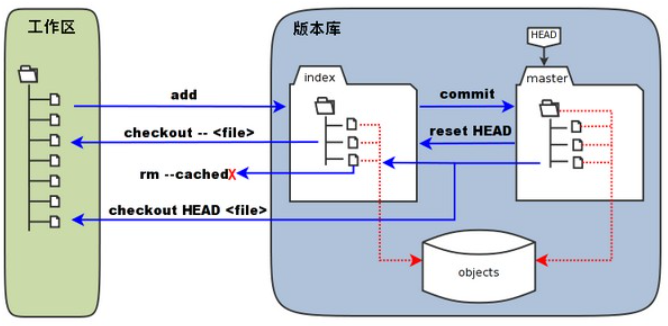
\includegraphics[scale=.6]{assets/git.png}};
			% \draw[help lines] (-7.5, -3.5) grid (7.5, 3.5);
			\node[fuchsia, fill=white] at (-3, 0.65) {\quad\texttt{restore \textcolor{gray}{[-W]}}\quad\ };
			\node[fuchsia, fill=white] at (-3.1, -1) {\quad\ \texttt{restore -S -W}\ \quad\ };
			\node[fuchsia, fill=gitbgblue] at (2.88, 0.69) {\texttt{restore -S}};
		\end{tikzpicture}
		\caption{Git 工作区、暂存区和版本库}
	\end{figure}

	\subsection{分支操作}

	\textcolor{maroon}{\textbf{强烈建议从 \url{https://learngitbranching.js.org/?locale=zh_CN} 学习!}}

	\textcolor{maroon}{\textbf{强烈建议从 \url{https://learngitbranching.js.org/?locale=zh_CN} 学习!}}

	\textcolor{maroon}{\textbf{强烈建议从 \url{https://learngitbranching.js.org/?locale=zh_CN} 学习!}}

	\begin{itemize}
		\itemsep0pt
		\item \texttt{git branch}:分支管理 (具体用法见 \texttt{git help branch})
		\item \texttt{git switch}:切换分支 (比较常见的 \texttt{git switch -c},创建并切换)
		\item \texttt{git tag}:标签管理 (\url{https://www.liaoxuefeng.com/wiki/896043488029600/900788941487552})
		\item \texttt{git log}:展示历史
		\item \texttt{git show}:显示提交内容\footnote{冷知识:\texttt{git log} 和 \texttt{git show} 的底层实现是完全一致的,只是默认选项不同而已。}
		\item \texttt{git diff}:显示版本间变化
		\item \texttt{git merge}:冲突处理之合并 (见前述链接)
		\item \texttt{git rebase}:冲突处理之变基 (见前述链接,其中 \texttt{git rebase -i} 较常用,可用于合并多个提交,简化版本树)
	\end{itemize}

	\subsection{远端操作}

	\begin{itemize}
		\itemsep0pt
		\item \texttt{git remote}:远端管理
		\item \texttt{git clone}:克隆远端仓库
		\item \texttt{git fetch}:收取远端变化
		\item \texttt{git push}:推送变化到远端
		\item \texttt{git pull}:\texttt{git fetch} + \texttt{git merge} (或 \texttt{git rebase})
		\item \texttt{git submodule}:子模块管理
	\end{itemize}

	分支跟踪:见 \cite{sast2021-git-2} 或 \texttt{git help branch}。

	\subsection{其他命令}

	这里还有一些\sout{可能在 Puzzle 中用得到的}命令,具体方法请自行使用 \texttt{git help} (记住,他们真的是很好的老师,我已经没什么好写的了)。

	\begin{itemize}
		\itemsep0pt
		\item \texttt{git blame}:查看贡献者 \sout{罪魁祸首 之 谁写的 bug}
		\item \texttt{git shortlog}:统计不同用户的贡献 \sout{找出摆烂的队友}
		\item \texttt{git reflog}:查询引用日志,用于误操作恢复
		\item \texttt{git bisect}:在版本树上二分查找定位 bug
		\item \danger\ \texttt{git gc} / \texttt{git prune} / \texttt{git fsck}:用于系统检查和垃圾清理
	\end{itemize}

	\subsection{Git 别名}
	\label{sss:gitalias}

	\textcolor{properpurple}{[\textit{直冲官方版:\url{https://git-scm.com/book/zh/v2/Git-\%E5\%9F\%BA\%E7\%A1\%80-Git-\%E5\%88\%AB\%E5\%90\%8D}}]}

	相信大家也可以发现,在平常使用 Git 时,经常会打出一长串又臭又长的命令,此时 Git 别名可以使使你的 Git 体验更简单、容易、熟悉。

	Git 的别名实际上就是节为 \texttt{alias} (键为 \texttt{alias.*}) 的配置,因此可以使用 \texttt{git config} 直接配置。由于 Git 别名通常给个人使用,因此配置时最好带上 \texttt{--global}。

	在下发的服务器的 \verb!~/.gitconfig! 文件中就有一些被注释掉的别名配置 (这些是我使用的),大家可以根据自己的需要定义别名。

	\subsection{gitignore}

	\textcolor{properpurple}{[\textit{直冲官方版:\url{https://git-scm.com/docs/gitignore} 或 \texttt{git help ignore}}]}

	在平时的工作中,经常会出现一些垃圾文件,如 C++ 的 \texttt{.o}, \texttt{.exe},LaTeX 的 \texttt{.log}, \texttt{.out},Node.js 的 \texttt{node\_modules},\sout{以及 macOS 的万恶之源\ \texttt{.DS\_Store}}。我们不希望这些 (可能很庞大) 的文件被 Git 跟踪 (或一不小心被加入暂存区甚至版本库),我们需要通过 Git 提供的 ignore-list 规则来告诉 Git 不需要管理的文件。

	简单地来说,你只需要在仓库的任意位置创建一个名为 \texttt{.gitignore} 的文件,然后一行写一个规则,使得满足这个规则的文件不被考虑。这样,你就可以放心使用 \texttt{git add .} 而不用担心加入奇奇怪怪的文件了。\cite{sast2021-git-2}

	.gitignore 文件的具体语法见 \url{https://git-scm.com/docs/gitignore#_pattern_format}。

	\begin{minted}[frame=single,linenos=true,rulecolor=blue,escapeinside=||]{shell}
# 忽略 folder 下的全部内容,这包括根目录下的 /folder/,也包括某个子目录下的 /child/folder/ 内容:
folder/*
# 忽略根目录下的 /folder/ 下的全部内容:
/folder/*
# 忽略所有 .cpp 文件:
*.cpp
# (尽管忽略所有 .cpp 文件,但) 不过滤 special.cpp 文件:
!special.cpp
	\end{minted}

	\danger\ 扩展:.gitignore 虽然能 ignore 掉一些文件,但其本身还是会被 Git 跟踪。有些时候你\sout{可能因为独特的环境}导致

	\hskip1.75em 产生一些只有你的工作区才有的脏东西,那么你不希望将它们添加到\ .gitignore 里。显然你不能把\ .gitignore 自己给 ignore 掉。此时,对于这一类文件,可以在 \texttt{\textcolor{fuchsia}./.git/info/exclude} 里填写,语法和\ .gitignore 相同。与 \hyperref[sss:gitconfig]{Git 配置}类似,它也有全局 (用户) 版本:\verb!~/.config/git/ignore!。

	\subsection[不通过 GitHub 直接交流]{\danger\ 不通过 GitHub 直接交流}

	一个常见的需求是你在写项目的时候需要和给你的分配某个服务器同步,然后本地写代码 (编辑起来比 Remote-SSH 快) 在服务器上调试运行 (有特定环境,有算力等)。

	此时一个常见的方法是通过 GitHub 去同步。但是这样就变成了中心化的方式,没有充分利用 Git 作为 DVCS 的优势。而 \texttt{rsync} 在这一方面又显得比较笨重,比如在增量更新,分支切换等方面。

	其实,\textbf{当你可以 SSH 一个服务器的时候,你就可以把它当成一个 SSH 协议的 Git 服务器!}具体操作如下 (假设你 SSH 使用的命令为 \texttt{ssh user@hostname},有端口的情况通过 \texttt{.ssh/config} 去掉):

	\begin{itemize}
		\itemsep0pt
		\item 设\textbf{远端}的仓库地址为 \texttt{/path/to/repository},建立一个空仓库或原仓库的副本 (第一次操作);
		\item 在\textbf{远端}的局部 (仓库) 配置上 \texttt{receive.denyCurrentBranch} 值为 \texttt{updateInstead} (\texttt{git help config} / \texttt{git help hooks});
		\item 然后在你\textbf{本地}的仓库中配置 \texttt{git remote add <name> user@hostname:/path/to/repository/.git};
		\item 这样就可以愉快地 \texttt{fetch}/\texttt{push} 啦!
	\end{itemize}

	\subsection{其他技巧}

	Git 还有很多小技巧,限于篇幅原因这里不一一介绍,有兴趣的同学可以查阅相关资料自行学习。

	\begin{itemize}
		\itemsep0pt
		\item Git LFS:用于管理大文件,如模型、数据等。\url{https://git-lfs.com/}
		\item 提交签名:给你的 Git 提交签名,这样你的提交就会旁边就会有 \textcolor{green!80!black}{Verified} 字样,防止别人伪造。\url{https://docs.github.com/zh/authentication/managing-commit-signature-verification}
		\item GitHub Actions:CI/CD 的好帮手,减轻人类的负担。
	\end{itemize}

	\section[实战]{$\overset{\text{zu\`o\vphantom y}}{\text{实}}\overset{\text{y\`e}}{\text{战}}$}

	\subsection{服务器连接}
	\label{sss:connserver}

	\textcolor{gray}{[\textit{前置技能:\texttt{ssh} 命令}]}

	我们会按照报名问卷的填写情况为大家分配服务器账号,在获取到你的服务器用户名、IP 地址与账号后,请使用以下命令连接到服务器:

	\begin{minted}[frame=single,linenos=true,rulecolor=blue,escapeinside=||]{shell}
ssh train@59.66.131.240 -p <port>
	\end{minted}

	所有人的初始账号均为 \texttt{train},初始密码均为 \texttt{sast2023}。具体的端口号 (即 \texttt{<port>} 一栏) 会通过 /* TODO */ 方式下发。

	\subsection{公钥登录 (推荐)}

	\textcolor{gray}{[\textit{前置技能:\texttt{ssh-keygen}, \texttt{ssh-copy-id} 命令}]}

	\textcolor{red}{在登录成功后请尽快配置公/私钥登录,并修改强密码或撤销密码登录,简要流程如下:}

	\begin{itemize}
		\itemsep0pt
		\item (在本地) 直接输入命令 \texttt{ssh-keygen} (注:可选参数 \texttt{-t ed25519},更多参数见命令手册),会在家目录的 \texttt{.ssh} 文件夹下生成一对公私钥 (\verb!id_rsa.pub! 和 \verb!id_rsa!)。
		\item (在本地) 运行 \texttt{ssh-copy-id train@59.66.131.240 -p <port>} (格式和 \hyperref[sss:connserver]{\ref*{sss:connserver} 节}相同,更多参数见命令手册),输入密码后即可完成 ``免密登录'' 配置。
	\end{itemize}

	\subsubsection{撤销密码登录 (可选)}

	\textcolor{gray}{[\textit{前置技能:\texttt{sshd} 服务相关原理}]}

	当你获得管理员 (\texttt{root}/\texttt{sudo}) 权限后,修改 \verb!/etc/ssh/sshd_config! 文件:

	\begin{itemize}
		\itemsep0pt
		\item 将第 57 (约) 行的 \verb!#PasswordAuthentication yes! 改为 \texttt{PasswordAuthentication no};
		\item 运行 \texttt{\textcolor{gray}{sudo} services ssh \textcolor{red}{reload}} 重新读取配置。
	\end{itemize}

	\subsection{CTF --- 简介}

	为保证趣味性,我们沿用之前几届的传统,采用 CTF (\href{https://en.wikipedia.org/wiki/Capture_the_flag_(cybersecurity)}{Capture the Flag}) 的形式进行。你需要在服务器环境中寻找格式形如 \textcolor{fuchsia}{\texttt{sast2023\{*******\}}} 的字符串,其中 \texttt{*******} 可以包含任何非空白 ASCII 可见字符。我们将这种字符串称为 ``flag''。每当你找到一个 ``flag''。你就可以通过 \hyperref[sss:ctfsubmit]{\ref*{sss:ctfsubmit} 节}中介绍的提交方式进行提交。\cite{sast2022-linux}

	\subsection{CTF --- 提交方式}
	\label{sss:ctfsubmit}

	\textcolor{gray}{[\textit{前置技能:简单的命令行网络工具,如 \texttt{curl}, \texttt{wget} 等}]}

	不提供额外的提交程序,请使用命令行发送网络请求的方式进行提交。推荐使用 \texttt{curl}。

	提交的命令如下 (尖括号 \textcolor{maroon}{\texttt< \texttt> \textbf 不}输入,花括号 \textcolor{maroon}{\texttt\{ \texttt\} \textbf 要}输入):

	\begin{minted}[frame=single,linenos=true,rulecolor=blue,escapeinside=||]{shell}
curl -d 'id=<你的学号>' -d 'flag=sast2023{*******}' http://59.66.131.240:50000/submit
	\end{minted}

	\vspace{-6pt}
	对于如外校等没有学号的用户,可以直接去掉学号一栏,即使用如下命令提交。此时该命令仅用于检测正确性,不提供累积计分与排名功能。

	\begin{minted}[frame=single,linenos=true,rulecolor=blue,escapeinside=||]{shell}
curl -d 'flag=sast2023{*******}' http://59.66.131.240:50000/submit
	\end{minted}

	\vspace{-6pt}
	输入该命令后,你的终端会返回你的提交是否有效。简单起见,如果返回以 \texttt{"Success":} 开头说明提交成功,否则会给出对应的错误信息。

	此外,你可以在浏览器直接访问 \url{http://59.66.131.240:50000/} 查看当前 ``flag'' 的获取情况以及排行榜。排行榜默认按照总分降序排列,同分按最后一次提交时间升序排列。你也可以点击表头更改排序方式。

	\subsection{CTF --- 注意事项与 FAQ}

	\begin{itemize}
		\itemsep0pt
		\item 所有的 ``flag'' 分为三大区:Linux, Git, Bonus,分别包含 9, 6, 6 个 ``flag'',占总数的 58, 36, 6 分。
		\item 藏匿的 ``flag'' 会以多种形式出现,\textit{一般而言},出现格式正确的字符串就是 ``flag'',除非有特殊说明,要求你寻找其中一个特定的 ``flag'' (这种现象在 Git 区中比较常见)。
		\item 欢迎与其他人交流讨论思路,以及向 ChatGPT/GPT-4 等工具求助。但请不要直接将 ``flag'' 告诉别人,这样会影响其他人的游戏体验。
		\item 提交 ``flag'' 的服务器和分配给你的服务器是同一个服务器,所以不要尝试做出伤敌一千自损八百的事情。
		\item 由于\raisebox{-3pt}{
\includegraphics{assets/pigeon.pdf}
\includegraphics{assets/pigeon.pdf}
\includegraphics{assets/pigeon.pdf}}的原因没做复杂的身份验证,所以请只用自己的学号提交 \sout{(真有人喜欢给别人送分吗?)}。
		\item ``mails'' 文件夹用于获得服务器的管理员权限以进行进一步操作,该文件夹与 ``flag'' 无关,且解锁所有三个区的 ``flag'' 都无需用到该权限 (即使用 ``train'' 账号即可完成)。
		\item 如果你没有分配到服务器,你可以去 Docker Hub 中 \url{https://hub.docker.com/r/jkjkmxmx/sast2023-linux-git} 下载原生的镜像来游玩,该镜像是 x86-64/amd64 架构的,最好保证你的计算机也是此架构 \sout{(好像用 arm64 的 QEMU 模拟会出现某些 flag 拿不到的问题)}。具体流程如下:
		\begin{minted}[frame=single,linenos=true,rulecolor=blue,breaklines=true]{shell}
docker pull jkjkmxmx/sast2023-linux-git
docker run --privileged -d -p 10000:22 -p 10001:80 -p 10002:3306 -p 10003:10001 -p 10004:10002 -h sast2023 --name sast2023 jkjkmxmx/sast2023-linux-git
ssh -p 10000 train@localhost
		\end{minted}
	\end{itemize}

	\subsection{CTF --- Linux 区}

	该区在 ``train'' 的家目录 (即 \texttt{/home/train}) 下的 ``puzzles'' 目录中进行。在这个目录中的每一个子目录 (如 ``envir'') 就代表一个谜题,\textbf{一个谜题恰对应一个 ``flag''}。

	每个谜题下一定存在一个\textit{与目录名同名}的可执行文件 (可以有多种形式:二进制文件,Shell 脚本等;以 ``envir'' 为例,即为 \texttt{envir/envir}),运行该文件并按照它的引导一步步获取 ``flag''。

	\subsection{CTF --- Git 区}

	该区在 ``train'' 的家目录下的 ``git'' 目录中进行。本区包含 6 个 flag,简要介绍如下:

	\subsubsection{Branches}

	\begin{itemize}
		\item 看看这个仓库里有哪些分支?
	\end{itemize}

	\subsubsection{Message}

	\begin{itemize}
		\item 提交信息不止只有标题哦,还有正文!
	\end{itemize}

	\subsubsection{History}

	\begin{itemize}
		\item 数据被覆盖了!看看怎么跳回之前的版本?
	\end{itemize}

	\subsubsection{Reflog}

	\begin{itemize}
		\itemsep0pt
		\item 该谜题在 ``reflog'' 分支下进行。
		\item 观察提交信息:``add correct Taylor formula'',这说明之前有可能加入了错误的公式。
		\item 但是它不在版本树里,这说明很可能被 \texttt{git reset} 过。那该如何恢复这样的 ``误操作'' 呢?
	\end{itemize}

	\subsubsection{Werewolf}

	\begin{itemize}
		\itemsep0pt
		\item 该谜题在 ``werewolf'' 分支下进行。
		\item \textbf{\textcolor{red}{state 文件下看起来有很多 ``flag'',但是这些基本都是假的。}}
		\item \textcolor{blue}{``预言家'' 告诉你:最终版本的所有 ``flag'' 中,唯一一个由 ``狼人'' (werewolf) 提供且没有被后面平民 (villager) 覆盖的 ``flag'' 才是真正的 ``flag''。}
	\end{itemize}

	\subsubsection{Debug}

	\begin{itemize}
		\itemsep0pt
		\item 该谜题在 ``debug'' 分支下进行。
		\item ``cat'' 对 \texttt{debug.cpp} 文件修改了很多次,但这些文件产生运行时错误了!``cat'' 想知道,究竟是哪一次提交,使这个程序第一次产生运行时错误呢\footnote{保证存在这样的提交,使得在其之前 \texttt{debug.cpp} 正常运行,它及其它之后均产生运行时错误。}?
		\item \textcolor{gray}{[\textit{该怎么寻找这样的提交呢?二分查找?如何在版本树中进行二分查找?}]}
		\item \textbf{\textcolor{properpurple}{只有这个提交正文里的 ``flag'' 才是真正的 ``flag'' 哦!}}
	\end{itemize}

	\subsection{CTF --- Bonus 区}

	该区会在任何可能的地方进行,它们\textit{有可能出现在服务器中,也有可能出现在其他任何地方}。作为彩蛋,这里不给出相关的提示,希望大家能开心地寻找。

	\section{致谢}

	本次作业参考了 2021 与 2022 年计算机系暑培 Linux 讲义与作业\cite{sast2022-linux}。本次作业镜像使用计算机系科协提供的 @Zeus 服务器进行分发,感谢它在 2\#-308B 日日夜夜勤勤恳恳地工作。本次作业的镜像上传到了 \href{https://hub.docker.com/r/jkjkmxmx/sast2023-linux-git}{Docker Hub},所编写代码将会在作业结束后全部开源,供后续培训设计时作为参考。

	\bibliographystyle{plain}
	\bibliography{handout}
\end{document}
